\documentclass[12]{article}

\usepackage[margin=1in]{geometry}
\usepackage{setspace}
\usepackage{graphicx}
\usepackage{verbatim}
\usepackage{amsmath}
\usepackage{ dsfont }
\usepackage{float}

\renewcommand{\baselinestretch}{1.15}

\begin{document} \noindent
401 project notes\\
\large
\textbf{Rough explanation of the paper}\\ \\ \normalsize
\textbf{Introduction}

	The setting: solving 2-D Laplace problems using rational function approximations, plus numerical experiments and examples.
	It turns out using rational function approximations with exponentially clustered points near singularities gets root-exponential convergence.
	
	Their problem:
	\begin{align*}
	\Delta u(z) &= \nabla^2 u(z) = \left( \frac{\partial^2}{\partial x^2} + \frac{\partial^2}{\partial y^2}\right)u(z) = 0,\enspace z\in \Omega \\ 		u(z)&=h(z),\enspace z\in \Gamma
	\end{align*}
in a domain $\Omega$ bounded piece-wise smoothly (with corners) by $\Gamma$, with specified boundary data $h$. This sort of problem comes up a lot in physics: electrostatics, fluid dynamics, heat conduction...
	
	The approach:
	\begin{align*}
	u(z)&\approx \mathrm{Re}[r(z)] \\
	r(z) &= \underbrace{\sum_{j=1}^{N_1} \frac{a_j}{z-z_j}}_\text{"Newman"} + \underbrace{\sum_{j=0}^{N_2} b_j (z-z_*)^j}_\text{"Runge"}
	\end{align*}
with poles ${z_j}$. The crux of the method is using exponentially clustered sample points on the boundary with $h$ near corners, along with exponentially clustered poles outside the boundary near the corners.
	
	The structure of the paper consists of: theorems establishing root-exponential convergence with rational approximations, then an algorithm using linear least-squares fitting on the boundary to find coefficients $a_j$ and $b_j$. 
	
	These are important facts:
	
	\textbf{Proposition} If $f$ is holomorphic, then its real and imaginary parts, $u$ and $v$ respectively, are harmonic. 
	
	\textbf{Proposition} If $f$ is harmonic, then all its partial derivatives are harmonic.
	
	\textbf{Prove $r(z)$ is harmonic (satisfies Laplace's eq.)} (SKETCH) Consider a very simple rational function $f(z)=1/z$. This function can be decomposed as $f(z)=u(x,y)+i\,v(x,y)$, where
	\begin{align*}
	u(x,y)=\frac{x}{x^2+y^2} &&
	v(x,y)=\frac{-y}{x^2+y^2}.
	\end{align*}
Taking derivatives will show that $u$ and $v$ satisfy the Cauchy-Riemann equations, which makes $f$ holomorphic and thus $u$ and $v$ harmonic. This result works the same for rational functions more of the form $f=1/(z-A)$ (via a variable substitution), emulating the "Newman" part of $r$. 

	Similarly, if we consider a simple polynomial $g(z)=(z-B)^k$ emulating the "Runge" part of $r$, we can determine that $g$ is holomorphic as well. It is simpler to use the polar form of $g$ in this case.
	
	Adding the two cases together and multiplying by constants is enough to show that $r$ must be holomorphic. We will use the real part of $r$, which must be harmonic, to approximate $u$.\\

\noindent
\textbf{Two Theorems}

	The theorems involve an analytic function $f$, while the applications involve a harmonic function $u$. However, and harmonic function $u$ can be the real part of an analytic function, i.e. $f=u+i v$.
	
	(***pictures***) $A_\theta=\{z \in \mathds{C} : |z|<1,\enspace |\mathrm{arg}(z)|<\theta \}$. The notation $||\cdot ||_\Omega$ is the supremum norm on $\Omega$.
	
	\textbf{(1)} Let $f$ be a bounded analytic function in the slit disk $A_\pi$ that satisfies $f(z)=O(|z|^\delta)$ as $z \to 0$ for some $\delta > 0$, and let $\theta \in (0,\pi /2)$ be fixed. Then for some $0< \rho < 1$ depending on $\theta$ but not on $f$, there exist type $(n-1,n)$ rational functions $\{r_n\}$, $1 \leq n < \infty$, such that
	\begin{align*}
	||f-r_n||_\Omega = O(e^{-C \sqrt{n}})
	\end{align*}
as $n \to \infty $ for some $C>0$, where $\Omega = \rho A_\theta$. Moreover, each $r_n$ can be taken to have simple poles only at
	\begin{align*}
	\beta_j = -e^{-\sigma j/\sqrt{n}}, \enspace 0\leq j \leq n-1,
	\end{align*}
where $\sigma >0$ is arbitrary.

	Translation: for a sufficiently well behaved function, we can get really good (root-exponential) approximations from some rational functions on a wedge domain like $A_\theta$. This is what the "Newman" part of the approximation is for. This is the first step towards the goal, as this gives us the good approximations on corner singularities. This theorem says that such rational functions exist, but does not describe how to construct them. The proof is based on using interpolation. 
	
	\textbf{(2)} Let $\Omega$ be a convex polygon with corners $w_1 , \ldots , w_m$, and let $f$ be an analytic function in $\Omega$ that is analytic on the interior of each side segment and can be analytically continued to a disk near each $w_k$ with a slit along the exterior bisector there. Assume $f$ satisfies $f(z)-f(w_k)=O(|z-w_k|^\delta)$ as $z \to w_k$ for each $k$ for some $\delta >0$. There exist degree $n$ rational functions $\{r_n\},\, 1 \leq n < \infty$ such that
	\begin{align*}
	||f-r_n||_\Omega=O(e^{-C\sqrt{n}})
	\end{align*}
as $n\to \infty$ for some $C>0$. Moreover, each $r_n$ can be taken to have finite poles only at points exponentially clustered along the exterior bisectors at the corners, with arbitrary clustering parameter $\sigma$, as long as the number of poles near each $w_k$ grows at least in proportion to $n$ as $n\to \infty$.

	Translation: for a sufficiently well behaved function, we can also get globally good approximations. The first theorem gives us the results near corners, and this one adds to that via the "Runge" part of the approximation.
	
	Some extensions: These same results hold for $\Omega$ bounded by analytic arcs meeting at corners. Additionally, the authors believe these results are valid also for non-convex domains and $\theta < \pi /2$. Experiments show that placing poles along exterior bisector is also not necessary.\\
	
\noindent
\textbf{Algorithm and Examples}

	Probably examples and pictures first... See \ref{fig:card pic} 
	\begin{figure}[H]
	\centering
	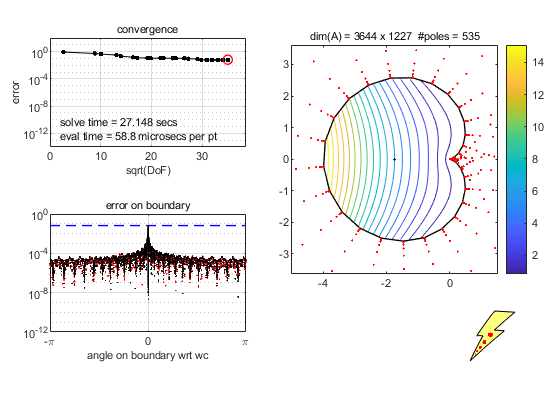
\includegraphics[scale=0.5]{cardioid.png}
	\caption{An example figure}
	\label{fig:card pic}
	\end{figure}
	
	The algorithm to construct the rational functions uses a least-squares, and specifically QR-factorization on a matrix of sample data to get the coefficients $a_j$ and $b_j$ from earlier.
	
	\begin{table}[h] The Algorithm \\
		\begin{tabular}{l}
			1. Define boundary $\Gamma$, corners $w_1,\ldots, w_m$, boundary function $h$, tolerance $\varepsilon$.	\\
			2. For increasing values of $n$ with $\sqrt{n}$	approximately evenly spaced; \\
			\: 2a. fix $N_1=O(mn)$ poles $1/(z-z_k)$ clustered outside the corners; \\
			\: 2b. fix $N_2+1=O(n)$ monomials $1,(z-z_*),\ldots,(z-z_*)^{N_2}$ and set $N=N_1+N_2+1$; \\
			\: 2c. choose $M\approx 3N$ sample points on a boundary, also clustered near corners; \\
			\: 2d. evaluate at sample points to obtain an $M\times N$ matrix $A$ and $M$-vector $b$; \\
			\: 2e. solve the least-squares problem $Ax\approx b$ for the coefficient vector $x$; \\
			\: 2f. exit loop if $||Ax-b||_\infty < \varepsilon$ or if $N$ is too large or the error is growing. \\
			3. Confirm accuracy by checking the error on a finer boundary mesh. \\
			4. Construct a function to evaluate $r(z)$ based on computed coefficients $x$.
		\end{tabular}
	\end{table}
	
	Possibly go deeper into a few of these steps... 
	
	Discussion of the code? Discussion of QR-factorization?
	
	An original example using their code on (my?) problem...



\end{document}